\section{Grundlegende Architektur}\label{sec:architecture}

\begin{wrapfigure}{r}{0.5\columnwidth}
	\centering
	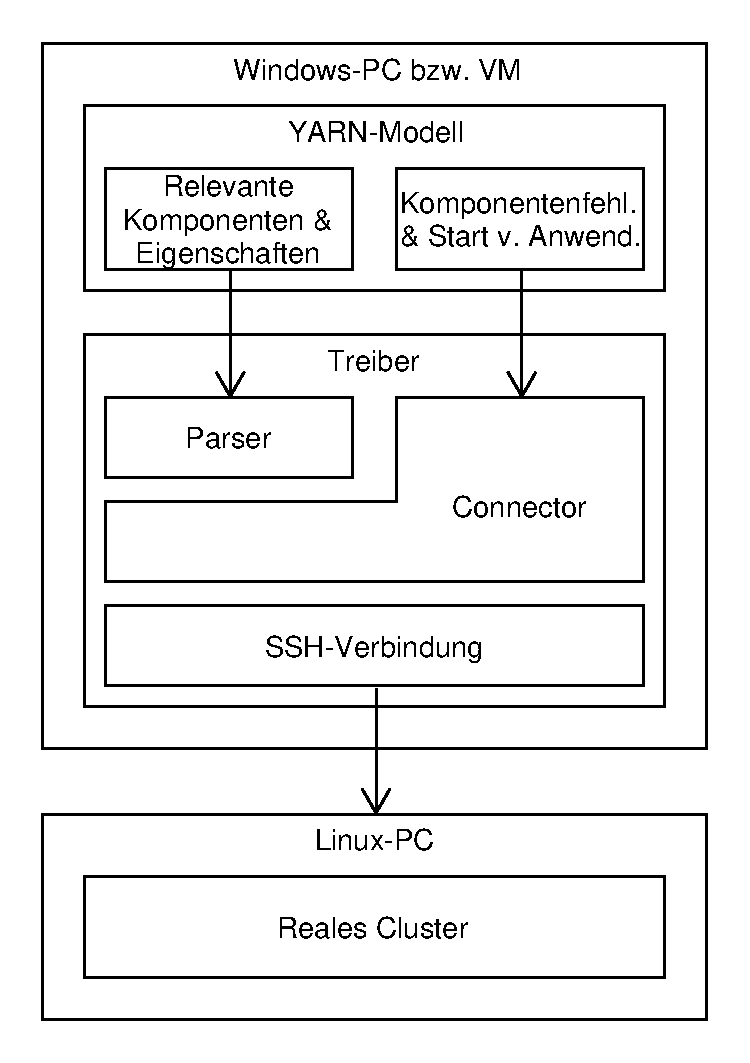
\includegraphics[width=0.5\columnwidth]{./images/modelArchitecture.pdf}
	\caption{Grundlegende Architektur des Gesamtmodells}
	\label{fig:modelArchitecture}
\end{wrapfigure}

Die grundlegende Architektur des gesamten Aufbaus besteht aus den drei rechts abgebildeten Schichten. Die oberste Schicht bildet das \sS-Modell von Hadoop YARN, welches die wesentlichen YARN-Komponenten und deren Komponentenfehler abbildet. Das reale Pendant dazu bildet das reale Cluster auf einem eigenen PC als unterste Schicht. Die Verbindung zwischen dem Modell und dem realen Cluster bildet der Treiber als eigenständige Schicht, bestehend aus dem Parser, Connector und der eigentlichen SSH-Verbindung zum zweiten PC mit dem realen Cluster.